\chapter{DUNE Calibration Strategy}
\label{ch:exec-summ-calib}

The DUNE \dword{fd} presents a unique challenge for calibration in many ways. Not only because of its size---the largest \dword{lartpc} ever constructed -- but also because of its depth. It differs both from existing long-baseline neutrino detectors, and existing \dwords{lartpc} (e.g. the deep underground location). While DUNE is expected to have a \dword{lartpc} as ND, DUNE is unlike previous long baseline experiments (MINOS, \dword{nova}) in that the near detector will have significant differences (pile-up, readout) that may make extrapolation of detector characteristics non-trivial.  %have a does not as yet have a near detector design and, unlike MINOS and \dword{nova}, the near detector is unlikely to be very much like the \dword{fd}. 
Like any \dword{lartpc}, DUNE has the great advantage precision tracking and calorimetry, but,  fully exploiting this capability requires a detailed understanding of the detector response. This challenge is driven by the inherently highly convolved detector response model and strong correlations that exist between various calibration quantities. For example, the determination of energy associated to an event of interest will depend on the simulation model, associated calibration parameters, non-trivial correlations between the parameters and spatial and temporal dependence of those parameters. These variations in parameters occur since the detector is not static. Changes can be abrupt (e.g. noise, a broken resistor in the field cage), or ongoing (e.g. exchange of fluid through volume, ion accumulation). 

A convincing measurement of CP violation, or a resolution of the neutrino mass ordering, or  \dword{snb} detection will require a demonstration that the overall detector response is well understood. %, and can be extrapolated across the entire physics regions of interest. 
This chapter describes a strategy for detector calibration for both 
\dwords{spmod} and \dwords{dpmod} using dedicated \dword{fd} systems or existing calibration sources. A large portion of the calibration work reported here is done under the joint \dword{sp} and \dword{dp} calibration task force formed in August 2017.
Section~\ref{sec:calibstrat} summarizes a calibration strategy currently envisioned for DUNE. The systematic uncertainties for the long baseline and low energy (supernova) program will determine how precisely each calibration parameter needs to be measured. For example, how precisely will the drift velocity need to be measured to know fiducial volume better than \num{1}\%? In general, the calibration program must provide measurements at the few percent or better level stably across an enormous volume and a long period of time. The calibration strategy must also provide sufficient redundancy in the measurement program.

Existing calibration sources for DUNE include beam or atmospheric neutrino-induced samples, cosmic rays, argon isotopes, and instrumentation devices such as liquid argon purity and temperature monitors. It is important for calibration strategy to further separate these sources into those used to measure a response model parameter, and those used to test the response model. In addition to existing sources, external measurements prior to DUNE will validate techniques, tools and design of systems applicable to the DUNE calibration program; data from  \dword{protodune} and SBND are essential to the success of the overall calibration program. %In addition to existing sources, calibration measurements and tools from other \dword{lar} experiments such as \dword{protodune} and SBN will be of critical importance for DUNE for early calibration when in-situ measurements in the FD will not be available.
Section~\ref{sec:exis} describes calibration from existing source of particles and external measurements.

%This includes both past measurements (e.g., ArgoNeuT, DUNE \dword{35t}, \dword{microboone}, LArIAT), anticipated measurements from ongoing and future experiments (e.g., \dword{microboone}, \dword{protodune}) as well as from small scale \dword{lartpc} test stands. \Dword{protodune} and previous measurements provide independent, critical tests of the response model, where the choice of parameterization and values correctly reproduces real detector data. However informative, not all of the previous ex-situ measurements will be directly extrapolatable to DUNE, only those that are believed to be universal (e.g. argon ionization energy). 

%Existing calibration sources for DUNE include (beam or atmospheric) neutrino-induced samples, cosmic rays, argon isotopes and instrumentation devices such as liquid argon purity and temperature monitors. While there are many existing calibration sources, each source comes with its own challenges. We further distinguish between sources which are used to measure a response model parameter, and measurements which test the response model. For example, electrons from 
%muon decay (Michel electrons) are very useful to study the detector response to low energy electrons ($\sim$ \SI{50}{\MeV}). However, low-energy electrons have major reconstruction challenges due to the loss of charge from radiative photons as demonstrated in \dword{microboone}~\cite{uBmichel}. In terms of source category, Michel electrons are considered as an important, independent, and necessary test of the TPC energy response model, and not as a measurement of a particular response parameter. Section~\ref{sec:exis} describes calibration from existing source of particles and external measurements. 

Section~\ref{sec:calibnew} describes dedicated external calibration systems currently under consideration for DUNE to perform calibrations that cannot be achieved fully from existing sources or external measurements. All the systems proposed are currently being actively discussed in the calibration task force and were agreed as important systems by the DUNE collaboration. Under current assumptions, the calibration strategy and proposed calibration systems described in this document are applicable to both \dwords{spmod} and \dwords{dpmod}. %In the case of \dword{dp}, one of the biggest challenges is the \SI{12}{\m} long single drift path and ion accumulation at the liquid-gas interface. 
Finally, Section~\ref{sec:calibsum} provides a summary along with future steps for calibration and a path to the \dword{tdr}. 

\section{Calibration Strategy}
\label{sec:calibstrat} %% 1 page
%    Strategy: Methods / procedure /hardware.
%    how will calibration proceed
DUNE has a broad physics program that includes long baseline neutrino oscillation physics, supernova physics, nucleon decay, and other searches for new physics. The physics processes that lead to the formation of these signals and the detector effects that influence their propagation must be carefully understood in order to perform adequate calibrations, as they ultimately affect the detector's energy response. Several other categories of effects can impact measurements of physical quantities such as the neutrino interaction model or reconstruction pathologies. %In this chapter, we take as a target that calibration, by itself, needs to be sufficient for DUNE's program; other issues that limit the physics program are out of scope and can only amplify the overall error budget. 
These other effects are beyond the scope of the \dword{fd} calibration effort and can only amplify the overall error budget.
In the reminder of this section, we briefly describe the physics-driven calibration requirements, including the calibration sources and systems required for the different stages of the experiment.
%and the strategy to deploy those sources and systems to address physics needs that evolve with detector operations.

\subsection{Physics Driven Calibration Requirements}

%\fixme{We may cut the first three? sentences and reference LBL table/plots with a single sentence,  sorry. Same for other sections. Check with editors.}
\textbf{Long-baseline physics:} In the physics volume of the DUNE CDR~\cite{Acciarri:2015uup}, Figure~3.23 shows that increasing the uncertainties on the \nue event rate from \num{2}\% overall 
%\footnote{This uncertainty is an uncorrelated normalization uncertainty on the far detector \nue rate in a four sample FD fit that assumes reasonable near detector constrains on flux and cross sections.} 
to \num{3}\% results in a \num{50}\% longer run period to achieve a 5$\sigma$ determination of CP violation for 50\% of possible values of \dword{cpv}. The CDR also assumes that the fiducial volume is understood at the 1\% level. Thus, calibration information needs to provide approximately 1-2\% understanding of normalization, energy, and position resolution within the detector. Later studies~\cite{ebias} expanded the simple treatment of energy  presented above. In particular, \num{1}\% bias on the lepton energy has a significant impact on the sensitivity to \dword{cpv}. 
A \num{3}\% bias in the hadronic state (excluding neutrons) is important, as the inelasticity  distribution for neutrinos and antineutrinos is quite different.  A different fraction of the antineutrino's energy will go into the hadronic state. Finally, while studies largely consider a single, absolute energy scale, relative spatial differences across the enormous DUNE \dword{fd} volume will need to be monitored and corrected; this is also true for changes that occur in time. A number of in-situ calibration sources will be required to address these broad range of requirements. Michel electrons, neutral pions and radioactive sources (both intrinsic and external) are needed for calibrating detector response to electromagnetic activity in the tens to hundreds of MeV energy range. Stopping protons and muons from cosmic rays or beam interactions form an important calibration source for calorimetric reconstruction and particle identification. \Dword{protodune}, as a dedicated test beam experiment, provides critical measurements to characterize and validate particle identification strategies in a 1~kt scale detector and will be an essential input to the overall program. Dedicated calibration systems, like lasers, will be useful to provide in-situ full volume measurements of electric field distortions. Measuring the strength and uniformity of the electric field is a key aspect of calibration, as  estimates of calorimetric response and particle identification depend on electric field through recombination. The stringent physics requirements on energy scale and fiducial volume also put similarly stringent requirements on detector physics quantities such as electric field, drift velocity, electron lifetime, and the time dependences of these quantities.

\textbf{Supernova burst and low-energy neutrino physics:} For this physics, the signal events present specific reconstruction and calibration challenges and observable energy is shared between different charge clusters and types of energy depositions. Some of the primary requirements here include calibration of absolute energy scale and 
%understanding of energy resolution (nominally at $\sim$\num{20}\% level, although better would be desirable for resolution of supernova spectral features), 
understanding and improving the nominal 20\% energy resolution, important for resolving spectral features of \dword{snb} events,
calibration of time and and light response of optical photon detectors, absolute timing of events and understanding of detector response to radiological backgrounds. Potential calibration sources in this energy range include Michel electrons from muon decays (successfuly utilized by ICARUS and \dword{microboone}~\cite{Acciarri:2017sjy}), which have a well known spectrum up to $\sim$50~MeV. Radiological sources provide calibrations of photon, electron, and neutron response for energies below \SI{10}{\MeV}. It is more challenging to find ``standard candles'' between 50~MeV and \SI{100}{\MeV}, beyond cosmic-ray muon energy loss. \Dword{protodune} could potentially be a test bed for various calibration strategies. One can imagine also ancillary studies of detector response using detectors such as LArIAT~\cite{Cavanna:2014iqa}, \dword{microboone}~\cite{Acciarri:2016smi}, and SBND~\cite{Antonello:2015lea}. % The ultimate calibration would be using a source of neutrinos from pion decay at rest, such as that available at the Spallation Neutron Source~\cite{Bolozdynya:2012xv}, which have energies up to \SI{50}{\MeV} with a well-understood spectrum. %KM cut, too speculative?

\textbf{Nucleon decay and other exotic physics:} The calibration needs for nucleon decay and other exotic physics are comparable to the \dword{lbl} program as listed before. Signal channels for light dark matter and sterile neutrino searches will be neutral current interactions that are background to the \dword{lbl} physics program. %The DUNE nucleon decay group has done studies of detection of the proton decay channel \ptoknubar, %$p\rightarrow K+ \overline{\nu}$,  where the kaon decays to a muon, which subsequently decays to a positron. %~\cite{protondecaywidths}. 
Based on the widths of $dE/dx$-based metrics of particle identification, qualitatively, we need to calibrate $dE/dx$ across all drift and track orientations at the few percent level or better, which is a similar target of interest as the \dword{lbl} effort.

\begin{dunefigure}[Categories of measurements provided by Calibration.]{fig:calibneeds}{Categories of measurements provided by Calibration.}
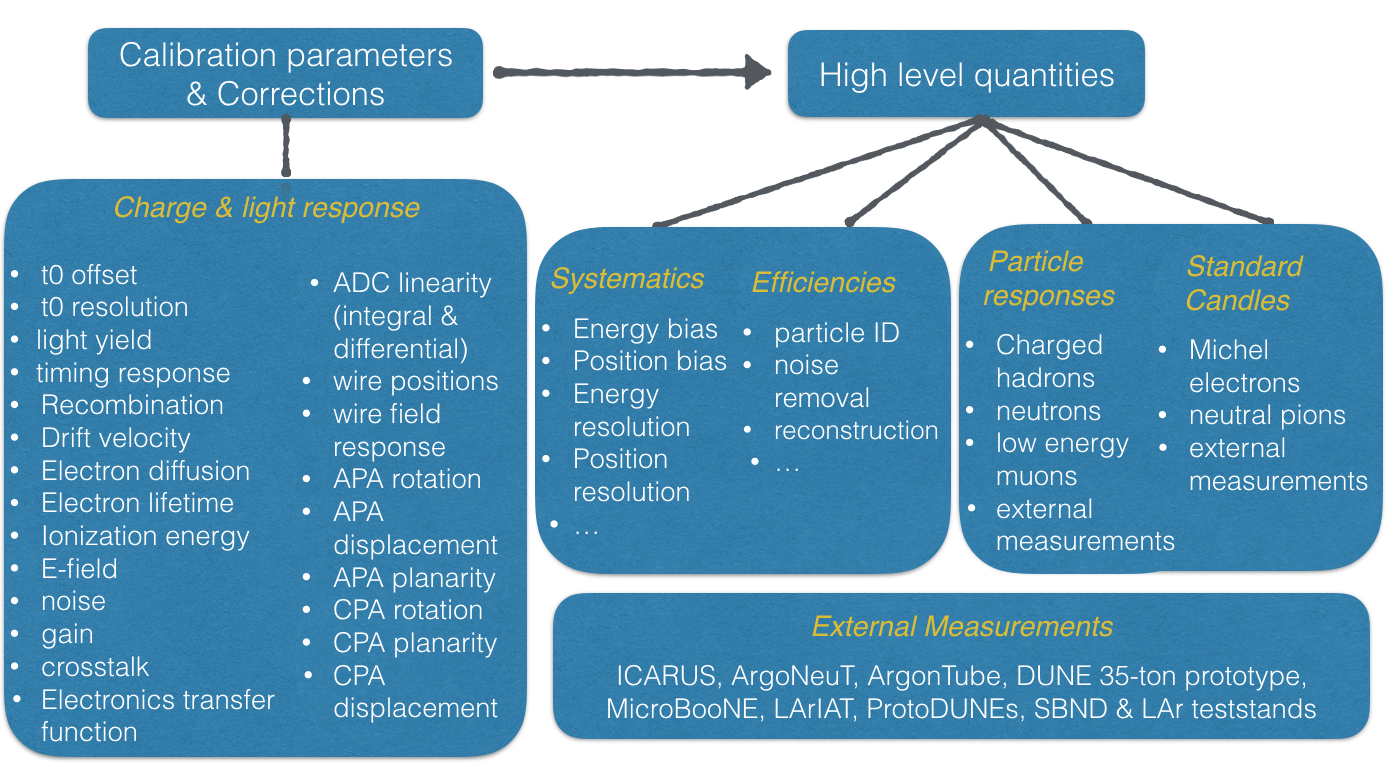
\includegraphics[width=.9\textwidth]{CalibNeeds_Final.png}
\end{dunefigure}

\textbf{Calibration Sources and Systems:} Calibration sources and systems provide measurements of the detector response model parameters, or provide tests of the response model. 
Calibration measurements can also provide corrections applied to data, data-driven efficiencies, systematics and particle responses. Figure~\ref{fig:calibneeds} shows the broad range of categories of measurements calibrations can provide and lists the critical calibration parameters for DUNE's detector response model applicable to both \dword{sp} or \dword{dp}. Due to the significant interdependencies of many parameters (e.g. recombination, electric field, liquid argon purity), a calibration strategy will either need to iteratively measure parameters, or find sources that break these correlations. Table~\ref{tab:calibsystem} provides a list of various calibration sources and proposed calibration systems along with their primary usage which will comprise the currently envisioned nominal DUNE FD calibration design to adequately address the needs for physics. More details on each of the calibration sources and systems are provided in the next sections. \Dword{protodune} and previous measurements provide independent, tests of the response model, where the choice of parameterization and values correctly reproduces real detector data, however not all of the ex situ measurements will be directly extrapolatable to DUNE due to other detector effects and conditions. Only those that are believed to be universal (e.g., argon ionization energy) can be extrapolated. Also, while there are many existing calibration sources, each source comes with its own challenges. For example, electrons from muon decay (Michel electrons) are very useful to study the detector response to low-energy electrons (\SI{50}{\MeV}). However, low-energy electrons present reconstruction challenges due to the loss of charge from radiative photons as demonstrated in \dword{microboone}~\cite{Acciarri:2017sjy}. In terms of source category, Michel electrons are considered as an important, independent, and necessary test of the TPC energy response model, and not as a measurement of a particular response parameter.

\begin{dunetable}[Calibration systems and sources of the nominal DUNE FD calibration design]
{p{.4\textwidth}p{.55\textwidth}}{tab:calibsystem}{Primary calibration systems and sources that comprise the nominal DUNE FD calibration design along with their primary usage.} 
%{ll}
% &  \\ \textbf{Usage} \toprowrule
System & \textbf{Primary Usage}  \\ \toprowrule 
\textbf{Existing Sources} & \textbf{Broad range of measurements} \\ \toprowrule
$\mu$, predominantly from cosmic ray & Position (partial), angle (partial) velocity (timing),  electron lifetime, wire response\\ \colhline % also timing offsets listed, related to drift velocity based on our discussion?
Decay electrons, $\pi^0$ from beam, cosmic, atm $\nu$ & Test of electromagnetic response model \\ \colhline
$^{39}$Ar &  electron lifetime (x,y,z,t), diffusion \\   \colhline 
\textbf{External Measurements} & \textbf{Tests of detector model, calibration techniques and systems} \\ \toprowrule
ArgoNeuT~\cite{Acciarri:2013met}, ICARUS~\cite{Amoruso:2004dy, Antonello:2014eha, Cennini:1994ha}, MicroBooNE & Model parameters (e.g. recombination, diffusion) \\ \colhline 
DUNE \dword{35t}~\cite{Warburton:2017ixr} & Alignment and \textit{t0} techniques\\ \colhline 
ArgonTUBE~\cite{Ereditato:2014tya}, MicroBooNE~\cite{Acciarri:2016smi}, SBND, ICARUS~\cite{Auger:2016tjc},  \Dword{protodune}~\cite{Abi:2017aow} & Test of systems (e.g. Laser, external muon taggers) \\ \colhline
ArgoNeuT~\cite{Acciarri:2015ncl}, MicroBooNE~\cite{bib:uBlifetime, MICROBOONE-NOTE-1018-PUB, MICROBOONE-NOTE-1028-PUB, Acciarri:2017sjy, Abratenko:2017nki, Acciarri:2013met}, ICARUS~\cite{Ankowski:2008aa,  Ankowski:2006ts,Antonello:2016niy},  \Dword{protodune} & Test of calibration techniques and detector model (e.g., electron lifetime, Michel electrons, $^{39}$Ar beta decays) \\ \colhline
\Dword{protodune}, LArIAT~\cite{Cavanna:2014iqa} & Test of particle response models and fluid flow models \\  \colhline
\dword{lartpc} test stands~\cite{Cancelo:2018dnf, Moss:2016yhb, Moss:2014ota, Li:2015rqa} & Light and LAr properties; signal processing techniques \\ \colhline 
\textbf{Monitoring Systems} & \textbf{Operation, Commissioning and Monitoring} \\ \toprowrule
Purity Monitors & Electron lifetime \\ \colhline
Photon Detection Monitoring System & \dword{pds} response \\ \colhline
Thermometers & Temperature, velocity; test of fluid flow model \\ \colhline
Charge injection & Electronics response \\ \colhline
\textbf{Proposed Systems} & \textbf{Targeted (near) independent, precision calibration}\\ \toprowrule
Direct ionization via laser & Position, angle, electric field (x,y,z,t) \\ \colhline
Photoelectric ejection via laser & Position, electric field (partial) \\ \colhline
Radioactive source deployment & Test of SN signal model \\ \colhline
Neutron injection & Test of SN signal, neutron capture model \\ \colhline
External Muon Tracker & Position, angle, muon reconstruction efficiency \\ \colhline
\end{dunetable}  

%\fixme{Are the systems on this table a complete list?}
%\fixme{I think we want a finite "fundamental parameter" list to reference. All of the above matters for energy estimator for a single track; fundamental and near fundamental measurements. Based on our earlier discussion I am using: angle of track, velocity, position, E field, recombination, diffusion, (electron) lifetime, temperature, LAr density, ionization energy, wire response, electronics response, impurity. We also have to relate timing to position, and emphasize spatial/temporal dependence and redundancy with this table. Sowjanya agree?}

\subsection{A Staged Approach}
The calibration strategy for DUNE will need to address the evolving operational and physics needs at every stage of the experiment in a timely manner using the primary sources and systems listed in Table~\ref{tab:calibsystem}. At the TDR stage, a clear and complete calibration strategy with necessary studies will be provided to demonstrate %the should be developed %that will meet the physics needs of the experiment in time along with an assessment of 
how the existing and proposed systems meet the physics requirements.
%This includes the realistic capabulity of the external and exis In particular, the capabil limitations of existing and external systems will be 
%with existing calibration sources, their limitations and what external calibration hardware systems will be needed for in-situ measurements. 
 Post-TDR, once the calibration strategy is set, necessary designs for calibration hardware along with tools and methods to be used with various calibration sources will need to be developed. To allow for flexibility in this process, the physical interfaces for calibration such as flanges or ports on the cryostat should be designed for a wide range of possible uses to accommodate the calibration hardware. As described in section~\ref{sec:FTs}, the calibration TF has made necessary accommodations for calibration systems for the \dword{spmod} in terms of feedthrough penetration design and will soon start finalizing the design and accommodations for calibration penetrations for the \dword{dpmod}. 

As DUNE physics turns on at different rates and times, a calibration strategy at each stage for physics and data taking is described below. This strategy assumes that all systems are commissioned and deployed according to the nominal DUNE run plan. 

\textbf{Commissioning:} When the detector is filled, data from various instrumentation devices will be needed to validate the argon fluid flow model and purification system. When the detector is filled and at desired high voltage, the detector immediately becomes live for supernovae and proton decay signals (beam and atmospheric neutrino physics will require a few years of data accumulation) at which stage it is critical for early calibration to track the space-time dependence of the detector. Noise data (taken with wires off) and pulser data (taken with signal calibration pulses injected into electronics) will be needed to understand the detector electronics response. Essential systems at this stage include temperature monitors, purity monitors, HV monitors, robust front-end charge injection system for cold electronics, and a PDS monitoring system for light. Additionally, as the $^{39}$Ar data will be available immediately, readiness (in terms of reconstruction tools and methods) to utilize $^{39}$Ar decays will be needed, both for understanding low energy response and space-time uniformity. External calibration systems as listed in Table~\ref{tab:calibsystem} will be deployed and commissioned at this stage and commissioning data from these systems will be needed to verify expected configuration for each system and any possible adjustments needed to tune for data taking.

\textbf{Early data taking:} Since DUNE will not have all in-situ measurements of liquid argon properties at this stage, early calibration of the detector will utilize liquid argon physical properties from \Dword{protodune} or SBND, and \efield{}s from calculations tuned to measured HV. This early data will most likely need to be recalibrated at a later stage when other data sets become available. This is expected to improve from in-situ measurements as data taking progresses and with dedicated calibration runs. The detector response models in simulation will need to be tuned on \Dword{protodune} and\slash or SBND data during this early phase, and the mechanism for performing this tuning needs to be ready. This together with cosmic ray muon analysis will provide an approximate energy response model that can be used for early physics. Analysis of cosmic ray muon data to develop methods and tools for muon reconstruction from MeV to TeV and a well-validated cosmic ray event generator with data will be essential for early physics. Cosmic ray or beam induced muon tracks tagged with an external muon tracker system will be very useful in these early stages to independently measure and benchmark muon reconstruction performance and efficiencies in the FD. Dedicated early calibration runs from external calibration systems will be needed to develop and tune calibration tools to data taking and correct for any space-time irregularities observed in the TPC system for early physics. Given the expected low rate of cosmic ray events at the underground location (see Section~\ref{sec:exis}), calibration with cosmic rays are not possible over short time scales and will proceed from coarse-grained to fine-grained over the course of years as statistics is accumulated. The experiment will have to rely on external systems such as laser for calibrations that require an independent probe with reduced or removed interdependencies, fine-grained measurements (both in space and time) and detector stability monitoring in the time scales needed for physics. Additionally some measurements are not possible with cosmic rays (e.g. APA flatness or global alignment of all APAs). 

\textbf{Stable operations:} Once the detector conditions are stabilized and the experiment is under stable running, dedicated calibration runs, ideally before, during and after each run period, will be needed to ensure detector conditions have not significantly changed. As statistics are accumulated, standard candle data samples (e.g. Michel electrons and neutral pions) both from cosmic rays, beam induced and atmospheric neutrinos can be used to validate and improve the detector response models needed for precision physics.  As DUNE becomes systematics limited, dedicated calibration campaigns using the proposed external systems will become crucial for precision calibration to meet the stringent physics requirements both for energy scale reconstruction and detector resolution. For example, understanding electromagnetic (EM) response in the FD will require both cosmic rays and external systems. The very high energy muons from cosmic rays at that depth that initiate EM showers (which would be rare at \Dword{protodune} or SBND), will provide information to study EM response at high energies. External systems such as radioactive sources or neutron injection sources will provide low energy EM response at the precision required for low energy supernovae physics. Other calibration needs not addressed with existing sources and external systems, will be determined initially from the output of the \Dword{protodune} and\slash or SBND program, and later from the DUNE ND if the design choice will be a LArTPC. 

%\fixme{We may want to be explicit about the external systems earlier in the strategy and explain their role more clearly here?} Fixed!

%\fixme{I am also making categories to separate measurements (of parameters in the detector response, listed above) and tests (of completeness of response model) }

%\fixme{Go through above for any reviewer comments; Xin had a comment about the nuances of protoDUNE re: impact of space charge on particle response. May need to revisit;} SG: fixed! see lines 7,8 and 9; KM like it?
%\fixme{What to put for charge injection system} Fixed!
%\fixme{CRT/EMT not included above, find a way to put it in.} Fixed!
